\scanpage{95}
\mspage{91}
% archive sheet number: 94

\uline{Proposition 4} Soit $\alpha:E\ \unsure{\text{---}|\longrightarrow}\ \unsure{\mathscr{P}|\mathcal{P}}(E')$ une correspondance, \deleted{\unsure{Considérons}} posons
\[
\begin{aligned}
\alpha' &: E\longrightarrow\Sigma_{E'},\qquad \alpha'(x)\overset{\text{\unsure{def|déf}}}=\operatorname{supp}^{\circ}_{E'}(\alpha(x))\\
\alpha_{\unsure{*|\ell}} &: \Sigma_E\ \unsure{\text{---}|\longrightarrow}\ \Sigma_{E'},
\end{aligned}
\]
\[
\deleted{\unsure{\alpha_*(S)}=\underset{x\in S}{\operatorname{Sup}_{\Sigma_{E'}}}\alpha'(x)=\underset{x\in S}{\unsure{\operatorname{Sup}}}\alpha'(x)}
\]
\[
\deleted{\unsure{\operatorname{supp}^{\circ}\bar\alpha(S)}}
\]
\[
\inserted{\alpha_*(S)=\operatorname{supp}^{\circ}_{E'}(\bar\alpha(S))=\underset{x\in S}{\operatorname{Sup}_{\Sigma_{E'}}}\alpha'(x).}
\]

Conditions équivalentes :

(i) $\alpha$ admet une prétransposée
\[
\beta:E'\longrightarrow\mathscr{P}(E)
\]
ou ce qui revient au $=$, une transposée
\[
\beta':E'\ \unsure{\longrightarrow|\text{---}}\ \Sigma_E,\quad\text{ou}\quad\beta_*:\Sigma_{E'}\ \unsure{\text{---}|\longrightarrow}\ \Sigma_E.
\]

\unsure{(ii)|(v)} \inserted{a)} $\alpha_*$ commute aux $\operatorname{Sup}$ quelconques.

\inserted{b) \deleted{\unsure{$\alpha$}} $\forall x\in E$,}
\[
\inserted{\alpha_*\operatorname{supp}^{\circ}_E(x)\ \bigl(\text{i.e. }\operatorname{supp}^{\circ}_{E'}(\bar\alpha(\operatorname{supp}^{\circ}_E(x)))\bigr)=\operatorname{supp}^{\circ}_{E'}(\alpha(x))}
\]

\deleted{\unsure{(iii)}}\unsure{(ii')|(iii)} On a les formules, pour \unsure{$\forall$} $A\in\mathscr{P}(E)$
\[
\alpha_*(\overbrace{\operatorname{supp}^{\circ}_E(A)}^{\bar A})=\operatorname{supp}^{\circ}_{E'}(\bar\alpha(A))
\]
(i.e. $\bar\alpha(\bar A)$ et $\bar\alpha(A)$ ont $=$ support dans $E'$)

\unsure{(iii)|(iv)} $\forall S'\in\Sigma_{E'}$, l'ens
\[
S=\{x\in E\mid\alpha'(x)\subset S'\}
\]
dans $E$ est dans $\Sigma_E$

(iv) $\forall x'\in E'$, l'ens
\[
\deleted{\unsure{\beta|\rho}}\inserted{\unsure{\gamma|\beta}}(x')=\{x\in E\mid\alpha(x)\mid\circ\mid x'\}
\]
est dans $\Sigma_E$.
% A long curved continuation arrow runs from condition (ii) to the foot of the page.

\figure{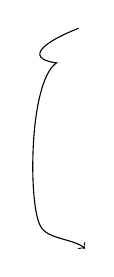
\begin{tikzpicture}[x=0.4cm,y=0.4cm]
\draw[->] (0.8,7) .. controls (-0.7,6.4) and (-0.7,6) .. (0.1,5.9) .. controls (-0.8,5.3) and (-0.8,1.3) .. (-0.4,0.7) .. controls (-0.2,0.3) and (0.7,0.3) .. (1,0);
\end{tikzpicture}}
